\chapter{Expérimentations}
\section{Donnés}\label{dataSet}
\paragraph{}Afin de tester notre programme nous avons opté pour l'utilisation de fichiers benchmark qui vont représenter des instances du problème, dorénavant, et pour être plus conforme avec la terminologie di problème, nous utiliserons le terme \textbf{INSTANCE} pour désigner ces dits fichiers.
\paragraph{}
Les instances nous sont présenté sous forme de fichiers au format \textbf{DIMACS}\footnote{Représentation convetionnelle d'une instance du problème SAT}(plus de détails dans \ref{par:dimacs}) et sont disponibles en téléchargement gratuitement et librement sur \cite{Benchmark}, et sont le fruit du travail de nombreux chercheurs dévoués.
\subsection{Format DIMACS}\label{par:dimacs}
Un fichier en format \textbf{DIMACS} est un fichier dont l'extension est \textbf{.cnf}, et est structuré de la manière suivante : \\\\ 
c\\
c start with comments\\
c\\
c \\

p cnf 5 3\\

1 -5 4 0\\
-1 5 3 4 0\\
-3 -4 0\\
\newpage
\paragraph{Explications :}
\begin{itemize}
	\item Le fichier peut commencer avec des commentaires, un commentaire sur une ligne commence par le caractère \textbf{"c"}
	\item La première ligne du fichier(après les commentaires) doit être structuré de la manière suivante : \textbf{p cnf nbvar nbclause}
	\begin{enumerate}
		\item \textbf{p cnf} pour indiquer que l'instance est en forme normale conjonctive \textbf{FNC}.
		\item \textbf{nbvar} indique le nombre de litéral au total dans l'instance, à noté que chaque literal $x_{i}$ sera représenté par son indice $i$.
		\item \textbf{nbclause} le nombre total de clause présentes dans l'instance.
	\end{enumerate}
	\item chaque ligne représente une conjonction de litéraux $(x_{i} \vert \lnot x_{i})$ indentifiés par un numero $i$, séparés par un blanc, et le 0 à la fin dénote la fin d'une ligne.
\end{itemize}
\subsection{Type d'instances}
Dans \cite{Benchmark} nous avons à notre disposition deux types d'instances pour chaque taille du problème : \\
\begin{itemize}
	\item Un ensemble d'instances satisfiable dans un fichier dénommé UF\textbf{XX}-\textbf{YY},\\avec \textbf{XX} = nombre de litéraux et \textbf{YY} = nombre de clauses
\end{itemize}
\section{Environement de travail}
\subsection{Machines}
\paragraph{}
Pour les tests nous avons utilisé deux machines pour chaques groupes d'instances, autrement dit une machine pour éffecutuer les tests sur un ensembles d'instances satisfiables \textbf{UF75-325}\cite{Benchmark} et une autre sur les instances contradictoires(non satisfiables) \textbf{UUF75-325}\cite{Benchmark}, les caractéristiques de chaques machines sont données dans les figures \ref{fig:machineA} et \ref{fig:machineB} suivantes : 
\begin{figure}[H]
	\centering
	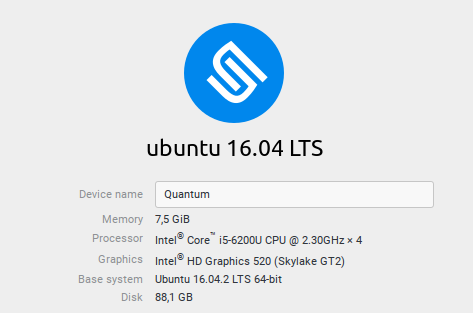
\includegraphics[scale=0.75]{images/machineWISS.png}
	\caption{Machine \textbf{A} pour les instances contradictoires}
	\label{fig:machineA}
\end{figure}
\begin{figure}[H]
	\centering
	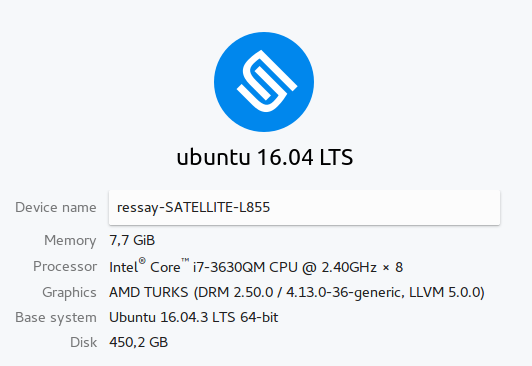
\includegraphics[scale=0.665]{images/machineYASSER.png}
	\caption{Machine \textbf{B} pour les instances satisfiables}
	\label{fig:machineB}
\end{figure}
\newpage
\subsection{Outils utilisés}
\subsubsection{Langage de programmation : }
\paragraph{}

\subsubsection{IDE : }
\paragraph{}
\paragraph{IntelliJ Idea} L'environement de dévelopement choisit est \href{URL}{IntelliJ IDEA}, spécialement dédié au développement en utilisant le langage \href{URL}{JAVA}, il est proposé par l'entreprise \href{https://www.jetbrains.com}{JetBrains} il est caractérisé par sa forte simplicité d'utilisation et les nombreuse plugins et extentions qui lui sont dédiées.

\section{Résultats}\label{tests}
\paragraph{}
\section{Statistiques}
\paragraph{}
\section{Comparaison entres les quatres méthodes}
\paragraph{}